\subsection{Draft Sequence}
\label{sec:draft-background}

The draft sequence comprises the processing stages that produce each capture's initial user-visible draft image.
It was introduced together with the post-processing pipeline, which produces the final image.
When post-processing completes, the final image replaces the draft image if one has already been published.
Figure~\ref{fig:draft-pipeline} illustrates this workflow.

The Draft pipeline uses a single worker to publish images in capture order and limit resource demand.
Executing multiple draft sequences concurrently would require buffering out-of-order results and increase peak compute and memory demand.

% Notes: docs/exhibits.md#fig_capture_pipeline
\begin{figure}[!ht]
  \centering
  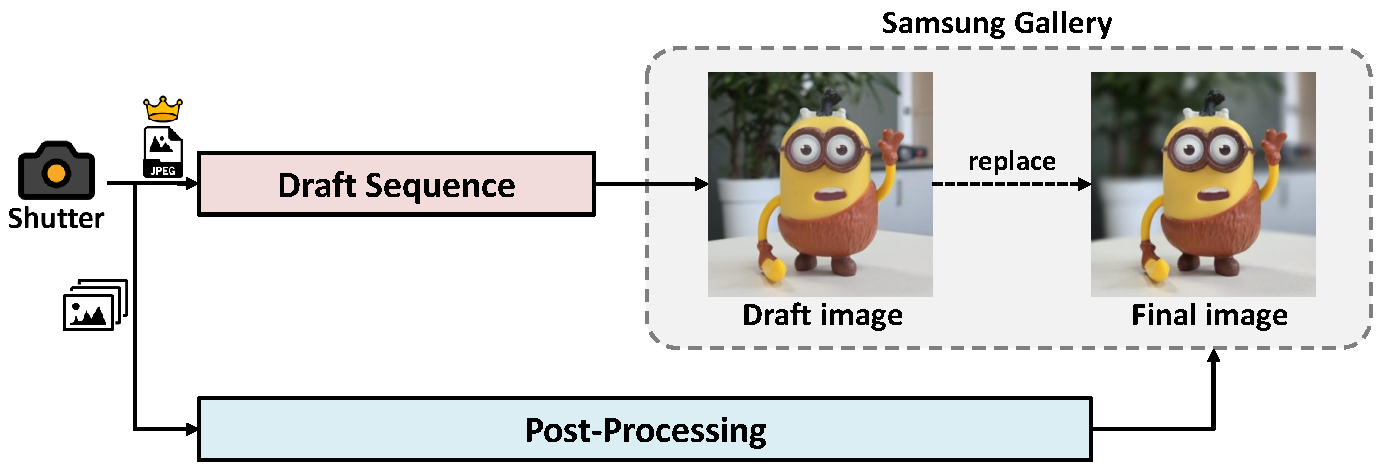
\includegraphics[width=\columnwidth]{figures/fig_capture_pipeline.pdf}
  \caption{Draft Sequence and Post-Processing.}
  \label{fig:capture-pipeline}
\end{figure}


\smallskip\noindent\textbf{Extending the Draft Sequence.}
The original draft sequence saved an image without additional image processing.
To reduce visual differences between draft and final images, the framework later added lightweight single-frame stages, such as Filter and Watermark.

As post-processing became more resource-intensive, the framework deferred its start for selected shot modes until the application entered the background to preserve foreground responsiveness.
In these modes, the draft image remains the user-visible result throughout the foreground session, making its visual quality more important.
The draft--final visual gap is particularly pronounced in Portrait mode.
To reduce this gap, we implemented lightweight multi-frame composition in the draft sequence.
However, the added processing time can cause Capture Timeout, so we have not deployed the feature on any device model.
Under parallel capture, this processing can also lengthen later captures' wait for the single draft worker.
